\documentclass{report}
\setlength{\headheight}{24.1638pt}
%packages
\usepackage[french]{babel}
\usepackage[T1]{fontenc}
\usepackage[utf8]{inputenc}
\usepackage{mathtools}
\usepackage{amssymb}
\usepackage{hyperref}
\usepackage{float}
\usepackage{amsthm}
\usepackage{listings}
\usepackage{geometry}
\usepackage{setspace}
\usepackage{graphicx}
\usepackage{fancyhdr}
\usepackage{subcaption}
\usepackage{cleveref}
\usepackage{tikz}
\usepackage{soul}
\usepackage{xcolor}
\begin{document}
\section{Interpolation par la méthode de Newton}
\subsection{Introduction}
La méthode de newton est une méthode d'interpolation qui permet de rendre le discret continu. C'est-à-dire que la méthode de newton peut établir, à partir d'un groupement de points, un polynome qui permet de tous les joindre. \\
\subsubsection{Quelques observations} \label{obs}
Pour comprendre au mieux cette méthode d'interpolation, nous remarquerons que le polynome d'interpolation peut s'écrire de la forme suivante:\\
\begin{center}
$P_{N-1}(x) = b_0 + b_1 (x-x_1) + b_2(x-x_1)(x-x_2)+ \ldots+b_{N-1}(x-x_1)\ldots(x-x_{N-1})$
\end{center}
Où $N$ est le nombre de points à interpoler. \\
$x_i, \forall i = 1,\ldots,N-1$ désigne l'élément i de la matrice des abscisses des points à interpoler  \\
et $b_i, \forall i=0,\ldots, N-1$, la $i^{\text{ème}}$ différence divisée. \\
\textit{On déduira alors que la méthode de Newton produira un polynome de degrè au plus N-1 pour N point}.\\


\subsection{Différence Divisée}
\textit{Dans cette section, $xi$ (respect. $y_i$ désigne l'abscisse (respect. l'ordonnée) du point $i$ et $b_i$ la $i^{\text{ème}}$ différence divisée}
Comme mentionné dans \ref{obs}, le polynome, pour exister, a besoin des \textbf{Différences Divisées}, notée \textit{$b_i$}.\\
Elles s'obtiennent en cherchant les coefficients $b_i$ tel que:
\begin{center}
$P_{N-1}(x_i) = y_i, \forall i=1,\ldots,N$
\end{center}
Cela revient à résoudre le système linéaire suivant:
\begin{center}
$
\begin{cases}
y_1 & = P_{N-1}(x_1) = b_0 \\
y_2 & = P_{N-1}(x_2) = b_0 + (x_2 - x_1) b_1 \\
\ldots&= \ldots  = \ldots \\
y_N &= P_{N-1}(x_N)= b_0 + (x_N - x_1)b_1+\ldots+(x_N-x_1)\ldots(x_N-x_{N-1})b_{N-1}
\end{cases}
$
\end{center}
\subsubsection{Notation}
On sythéthisera le système obtenu précédemment ainsi: \\
\begin{center}
La différence divisée $i$ de degrès $k$: $\bigtriangledown^{k}y_i = \frac{\bigtriangledown{k-1}y_i -\bigtriangledown^{k-1}y_k}{x_i - x_k}, i= k+1, \ldots, N.  $
\end{center}
\subsubsection{Conséquences}
Le coefficient $b_i$ est donc calculable ainsi:
\begin{center}
$b_i =
\begin{cases}
y_1 \text{ si } i=0  \\
\bigtriangledown^{i}y_{(i+1)} \forall i = 1,\ldots, N-1
\end{cases}
$
\end{center}
La seconde conséquence est la réecriture du polynome comme suit:\\
\begin{align*}
&P_0(x) = b_{N-1} \\
&P_1(x) = b_{N-2} + (x-x_{N-1})P_0(x) \\
&\ldots = \ldots \\
&P_{N-1}(x) = b_0 + (x-x1)P_{N-2}(x)
\end{align*}
\subsubsection{Remarque}
Le système de calcul de la différence divisée peut être visualiser comme une liste où on peut écraser l'élément $k$ par sa différence divisée.\\
Ceci nous sera utile lors de l'implémentation (utilisation de tableau et non de matrice).
\newpage
\subsection{Résolution Manuelle}
\begin{center}
    \textbf{Mettons en application la méthode de newton}\vspace{6pt}\\
\begin{tabular}{|c|c|c|c|}
    \hline
    $x_i$ & 2 & 6 & 4 \\
    \hline
    $y_i$ & 4 & 1.5 & -2\\
    \hline
\end{tabular}
\end{center}
\underline{\textit{Calcul des différences divisées}}\\
\begin{center}
    \begin{align*}
     &\bigtriangledown^{1}y_{(1)} = \frac{y_1 - y_0}{x_1-x_0} = -0.625 \\
     &\bigtriangledown^{1}y_{(2)} = \frac{y_2 - y_0}{x_2-x_0} = -3 \\
     &\bigtriangledown^{2}y_{(2)} = \frac{\bigtriangledown y_2 - \bigtriangledown y_1}{x_2-x_1} = 1.1875
    \end{align*}
\end{center}
\underline{\textit{Tableau des différences divisées}}\\
\begin{center}
$
\begin{array}{|c|c|c|c|}
\hline
x & y & \bigtriangledown & \bigtriangledown^2 \\
\hline
2 & 4 = b_0 &  & \\
\hline
& & -0625= b_1 &  \\ 
\hline
6 & 1.5&  & \\
\hline
& & & 1.1875 = b_2 \\
\hline
& &-3 & \\
\hline
4& -2 & & \\
\hline
\end{array}
$
\end{center}
\underline{\textit{Calcul du polynôme}}\\
\begin{center}
    \begin{align*}
    &P_0 (x) = b_2 = 1.1875 \\
    &P_1(x) = -0.625 + (x-6) \times P_0 = 1.1875x - 7.75 \\
    &P_2(x) = 4+ (x_2 )P_1 = 1.1875x^2-10.125x+19.5 
    \end{align*}
\end{center}
Le polynome interpolateur du groupement de points donné est donc le trinome:
\begin{center}
    $P_2(x)=1.1875x^2-10.125x+19.5$\\
\end{center}
\subsection{Algorithme}
Nous allons donc détailler les principales fonctions qui permettront par la suite l'implémentation de la méthode.
\textit{Dans toute cette section, $X$, $Y$, $DD$, $E$, $ne$, $XN$ et $P$ désigneront respectivement: les abscisses des points à interpoler, les ordonnées des points à interpoler, le tableau des différences divisées, Le tableau contenant l'evaluation du polynome sur un espace linéairement réparti, le nombre de nombre à générer de manière équitable sur un intervalle, un tableau contenant l'intervalle lineaire, un tableau contenant les coefficients du polynome}
\begin{lstlisting}[mathescape=true, frame=single, basicstyle=\linespread{1.5}\fontsize{8}{10}\selectfont, caption="Divided Difference function"]
Fonction DividedDifference(X, Y, DD):
   DD $\leftarrow$ Y
   n $\leftarrow$ X.length()
   for i from 0 to n-1:
   	   for j from n-1 to i+1 by step of -1:
   	   		DD[j] $\leftarrow \frac{D[j] - D[j-1]}{X[j] - X[j-i-1]}$
		end
    end
\end{lstlisting}
\begin{lstlisting}[mathescape=true, frame=single, basicstyle=\linespread{1.5}\fontsize{8}{10}\selectfont, caption="interpolate function"]
Fonction double interpolate(DD,X,x):
   double eval $\leftarrow 0$
   n $\leftarrow$ X.length()
   for i from n to 0 by step of -1:
   		eval $\leftarrow eval \times (x-X[i]) + DD[i]$
   	end
   	return eval
\end{lstlisting}
\begin{lstlisting}[mathescape=true, frame=single, basicstyle=\linespread{1.5}\fontsize{8}{10}\selectfont, caption="find coefficient function"]
Fonction coef(P, DD, X):
   n $\leftarrow$ X.length()
   P[0] $\leftarrow$ DD[n-1]
   for i from n-2 to 0 by step of -1:
   		for j from n-i-1 to j+1 by step of -1:
   			P[j] $\leftarrow$ P[j-1] -X[i] $\times$ P[j]
   		end
   	P[0] $\leftarrow$ DD[0] - X[i] $\times$ P[0]
   	end
\end{lstlisting}
Il s'agit uniquement de l'implémentation de la formule suivante:
\begin{center}
 $P_{N-1}(x) = b_0 + (x-x1)P_{N-2}(x)$
\end{center}
Pour générér un espace linéairement peuplé en fonction de $ne$, on générera les nombres ainsi:
\begin{lstlisting}[mathescape=true, frame=single, basicstyle=\linespread{1.5}\fontsize{8}{10}\selectfont, caption="generate linear space"]
some code:
for i from X[0] to X[X.length-1] by step of $\frac{max(X) - min(X)}{ne}$
some code
\end{lstlisting}
\subsection{Implémentation en C}
Pour implémenter l'interpolation de newton, nous utiliserons ces préceptes:
\begin{itemize}
\item Les données seront stockées sous notation scientifique (pour ne pas avoir d'erreur d'arrondie lors de l'utilisation en python
\item Le type polynome qui est un composée d'un entier \textbf{deg} et d'un tableau de coefficient double.
\item l'obtention du polynome d'interpolation sera comparé avec le resultat produit par sympy
\item Le programme prend 3 paramètres: le fichier input, le fichier output et enfin un entier qui déterminera en combien de morceau équitable voulons nous ségmenter l'intervalle $[X[0], X[X.length-1]]$ 
\end{itemize}
\newpage
\subsection{Exemples d'exécution}
Voici les différentes sorties du programme pour l'interpolation des jeux de données présents en annexe de ce document. Vous trouverez également un graphe représentant les points donnés, ainsi que le polynôme trouvé.
\begin{lstlisting}[caption={Annexe 1 data} results, basicstyle=\fontsize{8}{10}\selectfont]
    Polynom
0.000000x^19 - 0.000000x^18 + 0.000000x^17 - 0.000000x^16 + 
0.000000x^15 - 0.000000x^14 + 0.000000x^13 - 0.000000x^12 + 
0.000001x^11 - 0.000025x^10 + 0.000361x^9 - 0.004044x^8 + 
0.035004x^7 - 0.229974x^6 + 1.116527x^5 - 3.842630x^4 + 
8.760551x^3 - 11.683978x^2 + 6.758180x^1 + 0.999870

Temps d'execution : 0.096877 secondes
\end{lstlisting}
\begin{figure}[h]
    \centering
    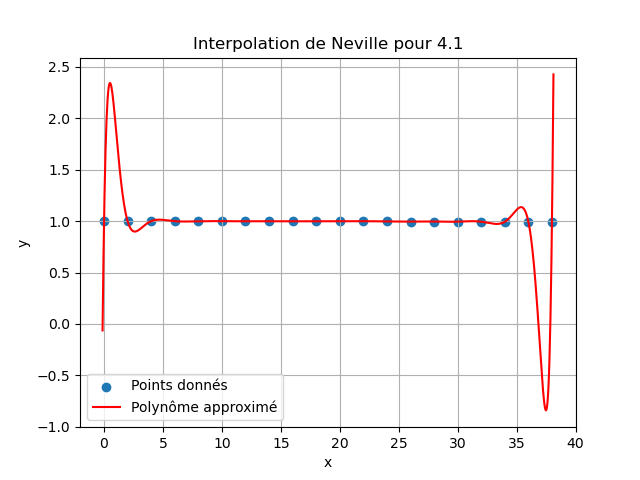
\includegraphics[width=0.7\textwidth]{sources/Corentin/polynomApproch/results/graphs/41.png}
    \caption{Interpolation du jeu de données 1 de l'annexe}
\end{figure}
\newpage
\begin{lstlisting}[caption={Annexe 2 data} results, basicstyle=\fontsize{8}{10}\selectfont]
    Polynom
0.000000x^20 - 0.000000x^19 + 0.000000x^18 - 0.000000x^17 + 
0.000000x^16 - 0.000000x^15 + 0.000000x^14 - 0.000000x^13 + 
0.000000x^12 - 0.000002x^11 + 0.001309x^10 - 0.860809x^9 + 
465.832642x^8 - 206286.906250x^7 + 74020648.000000x^6 - 
21189636096.000000x^5 + 4725708685312.000000x^4 
- 791294909612032.000000x^3 + 93583403189796864.000000x^2 - 
6969840492355780608.000000x^1 + 245843147369784279040.000000

Temps d'execution : 0.196364 secondes
\end{lstlisting}
\begin{figure}[h]
    \centering
    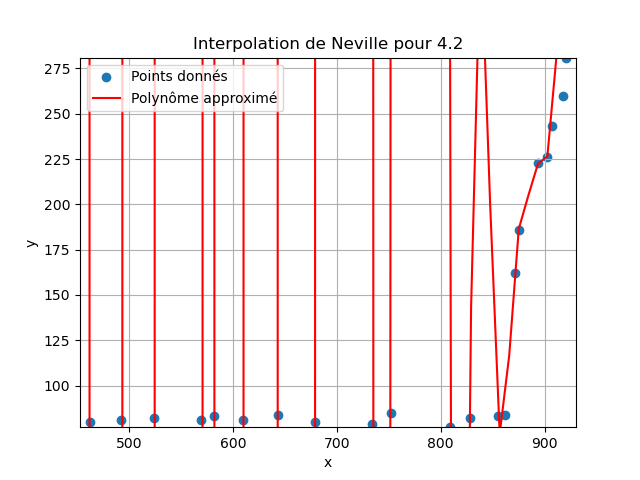
\includegraphics[width=0.7\textwidth]{sources/Corentin/polynomApproch/results/graphs/42.png}
    \caption{Interpolation du jeu de données 2 de l'annexe}
\end{figure}
\newpage
\begin{lstlisting}[caption={Annexe 3 data} results, basicstyle=\fontsize{8}{10}\selectfont]
    Polynom
0.000012x^10 - 0.001164x^9 + 0.049084x^8 - 1.220944x^7 + 
19.789038x^6 - 217.668701x^5 + 1639.865601x^4 - 
8326.726562x^3 + 27183.572266x^2 - 51370.457031x^1 + 42569.960938

Temps d'execution : 0.000282 secondes
\end{lstlisting}
\begin{figure}[h]
    \centering
    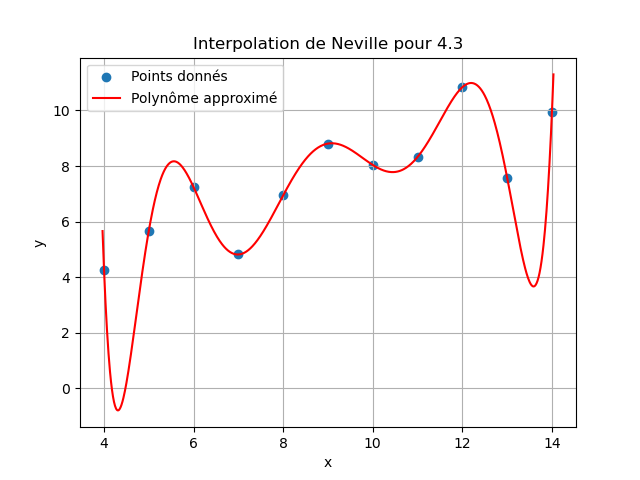
\includegraphics[width=0.7\textwidth]{sources/Corentin/polynomApproch/results/graphs/43.png}
    \caption{Interpolation du jeu de données 2 de l'annexe}
\end{figure}
\newpage
\end{document}